\documentclass[11pt,a4paper]{article}
\usepackage[margin=1in]{geometry}
\usepackage{amsmath,amssymb}
\usepackage{graphicx}
\usepackage{booktabs}
\usepackage{array}
\usepackage{tabularx}
\usepackage{enumitem}
\usepackage{float}
\usepackage{hyperref}
\usepackage{xcolor}
\usepackage{caption}
\usepackage{microtype}

\hypersetup{colorlinks=true,linkcolor=blue,urlcolor=blue,citecolor=blue}
\setlength{\parskip}{0.45em}
\setlength{\parindent}{1.5em}
\captionsetup{font=small}
\sloppy

\title{Detecting Initial /g/, /b/, /d/, and /z/ in MSWC English:\\
\large A Course-Constrained Spectral Template Method with Extended Baselines}
\author{Heng Qiao}
\date{April 29, 2026}

\begin{document}
\maketitle

\begin{abstract}
This report reformulates VE216 Project Topic 2 as a controlled initial-consonant detection problem. From MSWC English, the subset keeps only words whose first letter is \texttt{g}, \texttt{b}, \texttt{d}, or \texttt{z} and whose first non-vowel ARPABET phone is the matching consonant. The resulting corpus contains 60 words and 3000 utterances. The main method, \texttt{strict\_course\_fft}, uses short-time framing, FFT magnitude spectra, maximum-energy blocks, normalized correlation, and a sliding maximum score. It reaches 0.343 exact-match accuracy on the four-way test set. An extended template method, \texttt{course\_filterbank\_corr}, adds log-mel localization, positive-negative templates, and envelope autocorrelation, raising exact-match accuracy to 0.550. A feature MLP reaches 0.527, while a small CNN reaches 0.320. The results show that /z/ is the easiest class because its frication persists over time, while /g/ is the hardest because its burst is short and sensitive to alignment. The main value of the study is an interpretable signal-processing pipeline that makes the acoustic evidence visible before comparing stronger baselines.
\end{abstract}

\noindent\textbf{Keywords:} speech analysis; voiced consonants; short-time Fourier transform; template matching; keyword spotting; MSWC.

\section{Introduction and Problem Formulation}

The original project asks for spectral analysis of voiced consonants and a program that detects selected letters in spoken words. This report treats the task as four-way initial-consonant recognition rather than general word recognition. Each recording is a one-second, 16 kHz waveform $x_i[n]$. The class set is
\[
C=\{g,b,d,z\}, \qquad y_i\in\{0,1\}^{|C|}.
\]
Every retained sample has exactly one target initial consonant. The code still uses a four-output interface so that the template methods, MLP, and CNN can share the same evaluation path. A method produces a score vector $s_i\in\mathbb{R}^{|C|}$, and the final label is decoded as
\[
\hat c_i=\arg\max_{c\in C}s_{i,c},\qquad
\hat y_{i,c}=\mathbf{1}[c=\hat c_i].
\]
Per-class thresholds are estimated on the development set for compatibility with the multi-output code, but all reported test results use the exclusive four-way decoding above.

The split policy follows the usual train/development/test separation. Training data estimate templates or model weights. Development data choose block length, thresholds, and early stopping. Test data are used once for the final tables. No phone-level boundaries are supplied, so every method must find the useful initial-consonant evidence inside a whole-word recording.

\subsection{Evaluation metrics}

Let $N$ be the number of test samples and $K=|C|$. Label-wise accuracy compares each class bit separately:
\[
\mathrm{LabelAcc}
=\frac{1}{NK}\sum_{i=1}^{N}\sum_{c\in C}\mathbf{1}[\hat y_{i,c}=y_{i,c}].
\]
For this one-hot task, label-wise accuracy is higher than ordinary accuracy because it also counts true negatives.

Exact-match accuracy requires the whole label vector to match:
\[
\mathrm{ExactMatch}
=\frac{1}{N}\sum_{i=1}^{N}\mathbf{1}[\hat y_i=y_i].
\]
Here it is the standard four-class accuracy, so the result tables treat it as the main metric.

For each label $c$, precision, recall, and F1 are
\[
P_c=\frac{TP_c}{TP_c+FP_c},\qquad
R_c=\frac{TP_c}{TP_c+FN_c},\qquad
F1_c=\frac{2P_cR_c}{P_c+R_c}.
\]
Macro-F1 averages the four class-level F1 scores:
\[
\mathrm{MacroF1}=\frac{1}{K}\sum_{c\in C}F1_c.
\]
This metric shows whether one consonant class is being sacrificed.

Micro-F1 pools the $TP$, $FP$, and $FN$ counts before computing F1:
\[
\mathrm{MicroF1}
=\frac{2\sum_c TP_c}{2\sum_c TP_c+\sum_c FP_c+\sum_c FN_c}.
\]
Samples-F1 computes F1 on each sample and then averages:
\[
\mathrm{SamplesF1}
=\frac{1}{N}\sum_{i=1}^{N}
\frac{2|Y_i\cap \hat Y_i|}{|Y_i|+|\hat Y_i|}.
\]
Because every ground-truth and predicted label vector contains one positive class, micro-F1, samples-F1, and exact-match accuracy coincide numerically. They remain in the tables to match the shared evaluation interface.

The report is organized around the most interpretable method first. \texttt{strict\_course\_fft} is the course-constrained baseline: short-time FFT magnitude spectra and normalized correlation. \texttt{course\_filterbank\_corr} is reported as an extended template comparison because it adds log-mel features, onset localization, negative templates, and autocorrelation. The MLP and CNN appear after the signal-processing methods as baselines, not as the definition of the task.

\section{Related Work}

The task studied here is closer to local acoustic-event detection than to large-vocabulary speech recognition. The classifier only needs to decide which initial voiced consonant begins a short word. That makes short-time spectral analysis and template matching a useful starting point.

\subsection{Short-time speech representations}

Davis and Mermelstein showed that speech front ends gain stability by replacing raw waveforms with short-time parameterized spectra\cite{davis1980}. The usual pipeline frames the waveform over tens of milliseconds, applies a window, transforms each frame, and keeps the frequency-domain energy pattern. This representation preserves releases, frication, and vowel transitions while reducing sensitivity to raw waveform phase.

Rabiner's HMM tutorial connects frame-level features with temporal modeling\cite{rabiner1989}. The relevant point for this report is that speech evidence moves over time. Even without using an HMM, an initial-consonant detector should search a short region near the beginning of the word rather than average the whole recording into one global descriptor.

\subsection{Why consonants need local evidence}

The four target classes have different time-frequency behavior. /g/, /b/, and /d/ are voiced stops with short releases and fast transitions. /z/ is a voiced fricative with longer high-frequency energy. Whole-word averaging can bury these cues under the following vowel and speaker variation. Wilkinson and Russell's TIMIT phone-recognition work also points to the value of local formant and boundary-related evidence for phone discrimination\cite{wilkinson2002}.

For that reason, the main method starts with the tools closest to the course material: short-time FFT, local magnitude spectra, and normalized correlation. More complex baselines are useful only after the acoustic evidence has been made explicit.

\section{Dataset Construction}

\subsection{Selection rule}

The subset is generated by \path{src/prepare_mswc_initial_gbdz_subset.py}. A word is kept only when both conditions hold:
\begin{quote}
The first letter is one of \texttt{g/b/d/z}, and the first non-vowel phone in CMUdict/ARPABET is the corresponding consonant \texttt{G/B/D/Z}.
\end{quote}
This rule turns a loose spelling-based task into a pronunciation-based initial-consonant task. It excludes words where the target letter appears in the spelling but does not define the first consonant sound.

\subsection{Corpus size}

\begin{table}[H]
    \centering
    \caption{Size of the pronunciation-filtered initial-consonant subset.}
    \label{tab:dataset}
    \begin{tabular}{lcccc}
        \toprule
        Label & Words & Train & Development & Test \\
        \midrule
        /g/ & 15 & 600 & 75 & 75 \\
        /b/ & 15 & 600 & 75 & 75 \\
        /d/ & 15 & 600 & 75 & 75 \\
        /z/ & 15 & 600 & 75 & 75 \\
        \midrule
        Total & 60 & 2400 & 300 & 300 \\
        \bottomrule
    \end{tabular}
\end{table}

The final corpus is balanced at the word and utterance levels. Each class contributes 15 words and 750 utterances, split as 600/75/75. The 300-sample test set therefore supports direct class-wise comparison without reweighting.

\section{Methods}

\subsection{Course-constrained short-time FFT template method}

\texttt{strict\_course\_fft} assumes that the initial consonant can be represented by a short local magnitude-spectrum prototype. Speaker identity, recording level, and the following vowel all introduce variation, so the method compares normalized spectral shape rather than raw energy.

For sample $i$, use frame length $L=20$ ms, hop size $H=10$ ms, and $N=512$ FFT points. The spectrum of frame $m$ is
\[
X_{i,m}[k] = \sum_{n=0}^{L-1} x_i[n+mH]w[n]e^{-j2\pi kn/N},
\qquad k=0,\dots,N-1,
\]
where $w[n]$ is a Hamming window. Only the one-sided magnitude spectrum is kept. For a candidate block starting at frame $r$ and spanning $M$ frames, the descriptor is
\[
P_i^{(r)}[k]
=\frac{1}{M}\sum_{m=0}^{M-1}
\frac{|X_{i,r+m}[k]|}{\max_{\kappa}|X_{i,r+m}[\kappa]|},
\qquad k=0,\dots,N/2.
\]
The block descriptor is then $L_2$-normalized.

Templates are estimated from the training data. For each class $c$, the method first chooses the maximum-energy $M$-frame block from each positive sample and calls it $P_i^{(\star)}$. The class template is the normalized average
\[
T_c=\frac{\sum_{i:y_i=c}P_i^{(\star)}}
{\left\|\sum_{i:y_i=c}P_i^{(\star)}\right\|_2}.
\]
The development set selects the block length from $M\in\{3,4,5,6\}$. The selected value is $M=3$, after which the final templates are re-estimated from train+development samples. This keeps the main method within the course boundary: framing, FFT, averaging, and normalized correlation.

At test time, every candidate block is compared with every class template:
\[
\rho_{i,c}^{(r)}
=\frac{\langle P_i^{(r)},T_c\rangle}
{\|P_i^{(r)}\|_2\|T_c\|_2},
\qquad
s_{i,c}=\max_r\rho_{i,c}^{(r)}.
\]
The predicted class is $\arg\max_c s_{i,c}$. Appendix~\ref{alg:strict-course} gives the reproducible algorithm.

Figure~\ref{fig:strict-template} shows the template construction. The left side gives representative training blocks near the class mean, while the right side gives the normalized average template for each consonant.

\begin{figure}[H]
    \centering
    
\includegraphics[width=0.95\textwidth]{figures/mswc_course_gbdz_local_patch_v1/strict_course_template_construction.png}
    \caption{Template construction for \texttt{strict\_course\_fft}: maximum-energy blocks are extracted from train+development samples and averaged by class.}
    \label{fig:strict-template}
\end{figure}

Figure~\ref{fig:strict-corr} shows one correlation search. The method scans local candidate blocks, computes one score curve per class, and keeps the maximum score for each label.

\begin{figure}[H]
    \centering
    
\includegraphics[width=0.95\textwidth]{figures/mswc_course_gbdz_local_patch_v1/strict_course_correlation_demo.png}
    \caption{Correlation search in \texttt{strict\_course\_fft}. The classifier searches local blocks and assigns each class its best normalized-correlation score.}
    \label{fig:strict-corr}
\end{figure}

\subsection{Extended template method with filterbanks and autocorrelation}

\texttt{course\_filterbank\_corr} keeps the template-matching idea but expands the feature design. It uses log-mel filterbanks, estimates an onset window, builds both positive and negative templates for each label, and adds envelope autocorrelation. The method tests whether more precise localization and contrastive class information improve the same initial-consonant task.

With 25 ms frames and 10 ms hops, the method computes a 40-bin log-mel vector
\[
L_i[m,q]=\log\left(\sum_k |X_{i,m}[k]|^2 B_q[k]+\epsilon\right),
\qquad q=1,\dots,40.
\]
Frame energy is
\[
e_i[m]=\log\left(\frac{1}{40}\sum_q \exp L_i[m,q]+\epsilon\right).
\]
A five-frame moving average smooths $e_i[m]$. The onset $o_i$ is the first frame whose smoothed energy exceeds the initial median baseline by 0.22. The local window has 16 frames, starts two frames before the onset, and is evaluated under three offsets $\Delta\in\{-2,0,2\}$:
\[
W_i^{(\Delta)}=
L_i[o_i-2+\Delta: o_i-2+\Delta+15,:].
\]

Each candidate window is split into $S=3$ segments. The feature vector concatenates raw segment means and segment means after subtracting the two-frame pre-onset baseline:
\[
\phi_i^{(\Delta)}=
\left[
\mu_1(W),\mu_2(W),\mu_3(W),
\mu_1(W-\bar W_{\mathrm{pre}}),\mu_2(W-\bar W_{\mathrm{pre}}),\mu_3(W-\bar W_{\mathrm{pre}})
\right].
\]
Each $\mu_s$ is 40-dimensional, so $\phi_i^{(\Delta)}\in\mathbb{R}^{240}$. The same window also yields a 24-lag normalized autocorrelation vector $a_i^{(\Delta)}$ from the energy envelope.

For class $c$, the training set yields four templates: positive and negative spectral templates $P_c^+$ and $P_c^-$, plus positive and negative autocorrelation templates $A_c^+$ and $A_c^-$. The score for offset $\Delta$ is
\[
\begin{aligned}
g_{i,c}^{(\Delta)}=&\;0.65\left[
\cos(\phi_i^{(\Delta)},P_c^+)-\cos(\phi_i^{(\Delta)},P_c^-)
\right]\\
&+0.35\left[
\cos(a_i^{(\Delta)},A_c^+)-\cos(a_i^{(\Delta)},A_c^-)
\right],\\
s_{i,c}=&\;\max_{\Delta\in\{-2,0,2\}}g_{i,c}^{(\Delta)}.
\end{aligned}
\]
The extra terms improve accuracy but make the method less course-constrained. For that reason, this report treats it as an extended comparison rather than the primary classroom method. Appendix~\ref{alg:course-filterbank} gives the algorithm.

\begin{figure}[H]
    \centering
    
\includegraphics[width=0.98\textwidth]{figures/mswc_course_gbdz_local_patch_v1/course_filterbank_template_contrast.png}
    \caption{Positive-negative template differences in \texttt{course\_filterbank\_corr}. Warm regions are closer to positive samples; cool regions are closer to negative samples.}
    \label{fig:course-template-contrast}
\end{figure}

\begin{figure}[H]
    \centering
    
\includegraphics[width=0.95\textwidth]{figures/mswc_course_gbdz_local_patch_v1/course_filterbank_localization_demo.png}
    \caption{Onset localization and offset scoring in \texttt{course\_filterbank\_corr}.}
    \label{fig:course-localization}
\end{figure}

\subsection{MATLAB correspondence}

The course-constrained method maps to \path{src/matlab_course_template_detector.m} and \path{src/matlab_course_spectrum_demo.m}. The core score is the normalized inner product
\[
\texttt{score}=\frac{\texttt{mag}^\top \texttt{template}}{\|\texttt{mag}\|_2\|\texttt{template}\|_2}.
\]
\path{src/matlab_case_demo.m} visualizes the four case clips and their template scores. The MATLAB scripts show the course idea directly; the Python experiment adds development-set block selection and train+development template estimation for the formal test run.

\section{Case Analysis and Visualization}

\subsection{Spectral templates of four representative words}

Figure~\ref{fig:matlab-spectra} shows the short-time FFT templates of four representative words in the MATLAB demonstration. The figure is not a training summary. Its purpose is to show the actual shape of the local templates.

\begin{figure}[H]
    \centering
    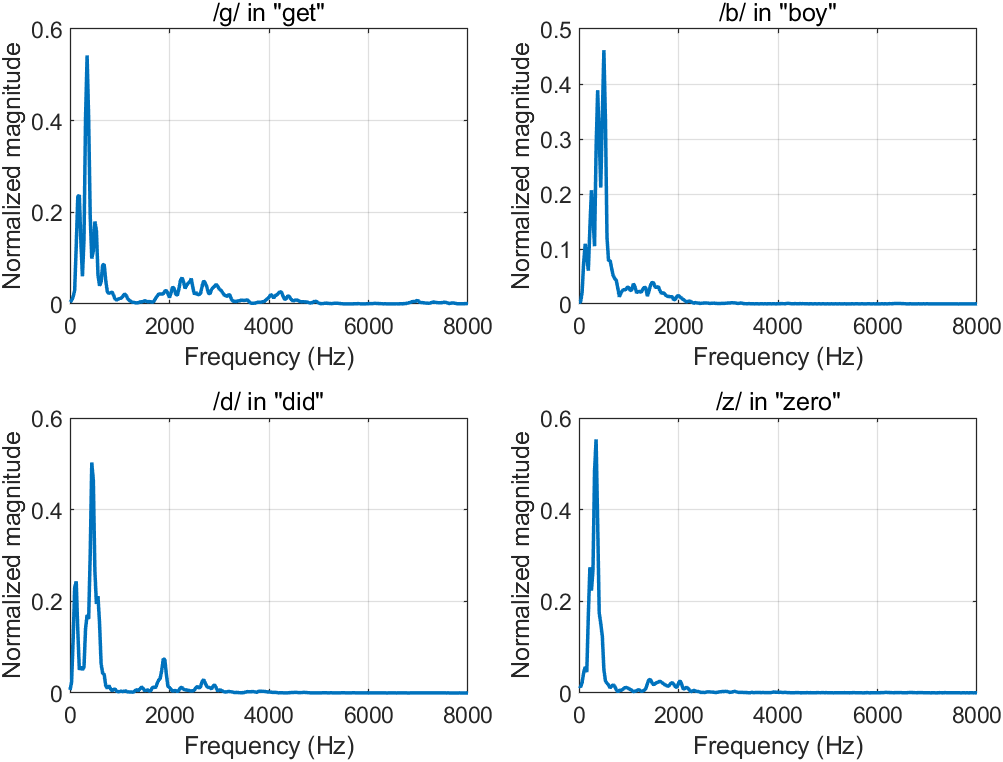
\includegraphics[width=0.95\textwidth]{figures/course_matlab/example_short_time_spectra.png}
    \caption{Short-time FFT magnitude templates of four representative words.}
    \label{fig:matlab-spectra}
\end{figure}

The figure shows a clear contrast. The high-frequency frication of /z/ lasts longer, the initial releases of /b/ and /d/ are shorter, and the short-time structure of /g/ is the easiest to blur when alignment shifts in time. This pattern is consistent with the class templates constructed by our method.

\subsection{Correlation score matrix}

Figure~\ref{fig:matlab-score} gives the correlation score matrix produced by the same set of templates on the four representative words. The figure is not meant to prove that the model is strong. It shows that the basic operation of template-query correlation is actually working.

\begin{figure}[H]
    \centering
    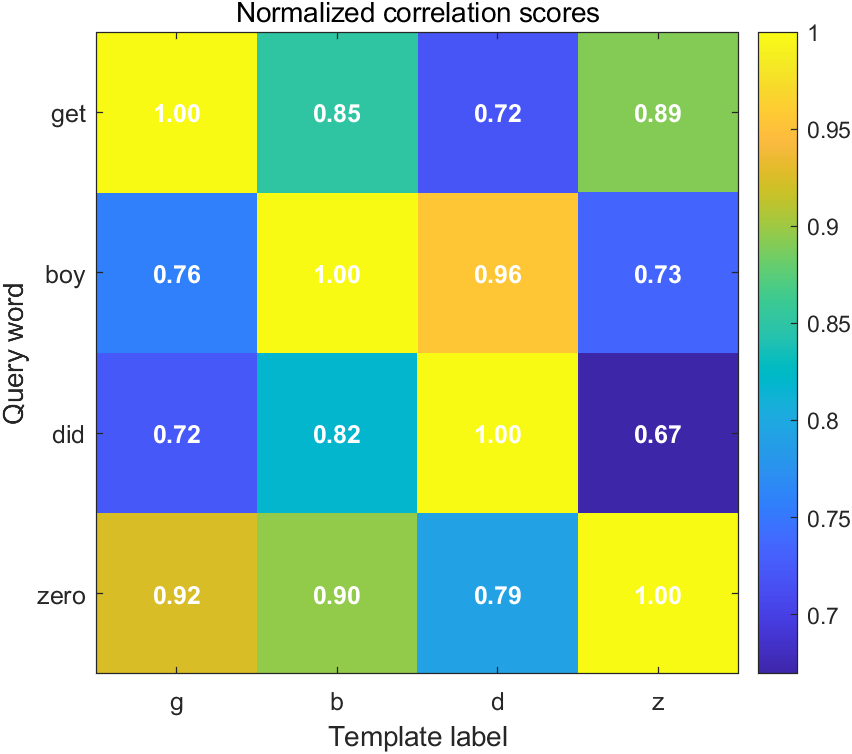
\includegraphics[width=0.70\textwidth]{figures/course_matlab/example_score_matrix.png}
    \caption{Correlation score matrix for four representative words.}
    \label{fig:matlab-score}
\end{figure}

This matrix is more direct than the waveform alone because it turns the question of which template looks most similar to a local speech segment into a numerical comparison. When the score gap is small, the alignment of the initial consonant is usually not stable enough. This is also the problem that the later AI reimplementation tries to address.

\section{Experimental Results}

\subsection{Course-constrained baseline}

The strict FFT template method is evaluated first because it is the main signal-processing baseline. In a one-hot four-class task, exact-match accuracy is the direct metric; label-wise accuracy is included only for consistency with the shared evaluation code.

The strict method uses two course-compatible refinements. It no longer builds templates from only the four case clips. Instead, it averages maximum-energy blocks from same-class training samples and then re-estimates the templates on train+development after choosing the block length. The development set selects a three-frame block.

\begin{table}[H]
    \centering
    \caption{Main metrics for the course-constrained FFT template method.}
    \label{tab:strict-main}
    \begin{tabular}{lccccc}
        \toprule
        Method & Label acc. & Exact match & Macro-F1 & Micro-F1 & Samples-F1 \\
        \midrule
        strict\_course\_fft & 0.6717 & 0.3433 & 0.3368 & 0.3433 & 0.3433 \\
        \bottomrule
    \end{tabular}
\end{table}

\begin{table}[H]
    \centering
    \caption{Per-label F1 for the course-constrained FFT template method.}
    \label{tab:strict-per-label}
    \begin{tabular}{lcccc}
        \toprule
        Method & /g/ & /b/ & /d/ & /z/ \\
        \midrule
        strict\_course\_fft & 0.250 & 0.377 & 0.345 & 0.375 \\
        \bottomrule
    \end{tabular}
\end{table}

Figure~\ref{fig:strict-score-dist} shows that positive and negative score distributions are separated but still overlap. The strict method captures meaningful spectral evidence, but the evidence is not strong enough for stable four-class recognition.

\begin{figure}[H]
    \centering
    \begin{minipage}{0.48\textwidth}
        \centering
        
\includegraphics[width=\linewidth]{figures/mswc_course_gbdz_local_patch_v1/strict_course/score_distribution_g.png}
        \small /g/
    \end{minipage}\hfill
    \begin{minipage}{0.48\textwidth}
        \centering
        
\includegraphics[width=\linewidth]{figures/mswc_course_gbdz_local_patch_v1/strict_course/score_distribution_b.png}
        \small /b/
    \end{minipage}

    \vspace{0.5em}
    \begin{minipage}{0.48\textwidth}
        \centering
        
\includegraphics[width=\linewidth]{figures/mswc_course_gbdz_local_patch_v1/strict_course/score_distribution_d.png}
        \small /d/
    \end{minipage}\hfill
    \begin{minipage}{0.48\textwidth}
        \centering
        
\includegraphics[width=\linewidth]{figures/mswc_course_gbdz_local_patch_v1/strict_course/score_distribution_z.png}
        \small /z/
    \end{minipage}
    \caption{Score distributions from \texttt{strict\_course\_fft} for the four labels.}
    \label{fig:strict-score-dist}
\end{figure}

\subsection{Extended template comparison}

\texttt{course\_filterbank\_corr} adds onset localization, log-mel positive-negative template differences, and envelope autocorrelation. These changes move beyond the strict course boundary, so the method is reported as an extended comparison.

\begin{table}[H]
    \centering
    \small
    \setlength{\tabcolsep}{4pt}
    \caption{Overall comparison between the course-constrained and extended template methods.}
    \label{tab:course-compare}
    \begin{tabular}{lccccc}
        \toprule
        Method & Label acc. & Exact match & Macro-F1 & Micro-F1 & Samples-F1 \\
        \midrule
        strict\_course\_fft & 0.6717 & 0.3433 & 0.3368 & 0.3433 & 0.3433 \\
        course\_filterbank\_corr & 0.7750 & 0.5500 & 0.5462 & 0.5500 & 0.5500 \\
        \bottomrule
    \end{tabular}
\end{table}

\begin{table}[H]
    \centering
    \caption{Per-label F1 for the course-constrained and extended template methods.}
    \label{tab:course-per-label}
    \begin{tabular}{lcccc}
        \toprule
        Method & /g/ & /b/ & /d/ & /z/ \\
        \midrule
        strict\_course\_fft & 0.250 & 0.377 & 0.345 & 0.375 \\
        course\_filterbank\_corr & 0.438 & 0.528 & 0.472 & 0.747 \\
        \bottomrule
    \end{tabular}
\end{table}

The extended method improves exact-match accuracy from 0.343 to 0.550. The largest gain appears for /z/, whose sustained frication is well matched by log-mel local templates and autocorrelation. /g/ remains the weakest class, consistent with its short burst and higher alignment sensitivity.

\begin{figure}[H]
    \centering
    
\includegraphics[width=0.95\textwidth]{figures/mswc_course_gbdz_local_patch_v1/letter_examples.png}
    \caption{Representative examples used by the extended template pipeline.}
    \label{fig:ext-examples}
\end{figure}

\begin{figure}[H]
    \centering
    
\includegraphics[width=0.90\textwidth]{figures/mswc_course_gbdz_local_patch_v1/template_grid.png}
    \caption{Average log-mel templates for the four classes. This view shows class-level energy patterns; it is separate from the positive-negative contrast templates used in scoring.}
    \label{fig:ext-template-grid}
\end{figure}

Figure~\ref{fig:course-score-dist} gives the test score distributions for the extended method. /z/ shows the clearest positive-negative separation. /g/, /b/, and /d/ still overlap, which explains why onset localization helps but does not remove stop-consonant confusion.

\begin{figure}[H]
    \centering
    \begin{minipage}{0.48\textwidth}
        \centering
        
\includegraphics[width=\linewidth]{figures/mswc_course_gbdz_local_patch_v1/course_filterbank_corr/score_distribution_g.png}
        \small /g/
    \end{minipage}\hfill
    \begin{minipage}{0.48\textwidth}
        \centering
        
\includegraphics[width=\linewidth]{figures/mswc_course_gbdz_local_patch_v1/course_filterbank_corr/score_distribution_b.png}
        \small /b/
    \end{minipage}

    \vspace{0.5em}
    \begin{minipage}{0.48\textwidth}
        \centering
        
\includegraphics[width=\linewidth]{figures/mswc_course_gbdz_local_patch_v1/course_filterbank_corr/score_distribution_d.png}
        \small /d/
    \end{minipage}\hfill
    \begin{minipage}{0.48\textwidth}
        \centering
        
\includegraphics[width=\linewidth]{figures/mswc_course_gbdz_local_patch_v1/course_filterbank_corr/score_distribution_z.png}
        \small /z/
    \end{minipage}
    \caption{Score distributions from \texttt{course\_filterbank\_corr} for the four labels.}
    \label{fig:course-score-dist}
\end{figure}

\section{Neural and Statistical Baselines}

The baselines in this section compare the template methods with two learned classifiers: a feature-based MLP and a small CNN. Both models train on the training split, use the development split for thresholding or early stopping, and report final metrics on the test split. Although the task is one-hot four-way classification, both models keep the same four-output interface as the template methods and use $\arg\max$ for the final label.

\subsection{MLP on MFCC and band-energy statistics}

The MLP does not take a full spectrogram as input. It uses a fixed vector of summary features. For each recording, the pipeline computes log-mel features, extracts 13 MFCC coefficients and their first-order differences, and concatenates
\[
z_i=
\left[
\mathrm{mean}(\mathrm{MFCC}),
\mathrm{std}(\mathrm{MFCC}),
\mathrm{mean}(\Delta\mathrm{MFCC}),
\mathrm{std}(\Delta\mathrm{MFCC}),
\mathrm{bandEnergy}
\right].
\]
The first four groups contribute $13\times4=52$ dimensions. The band-energy block contributes 10 more, so $z_i\in\mathbb{R}^{62}$. The features are standardized with the training-set mean and variance.

The network has two hidden layers:
\[
h_1=\mathrm{ReLU}(W_1z_i+b_1),\qquad
h_2=\mathrm{ReLU}(W_2h_1+b_2),\qquad
p_i=\sigma(W_3h_2+b_3),
\]
with widths 128 and 64. The loss is binary cross entropy over the four output labels plus $L_2$ regularization:
\[
\mathcal{L}_{\mathrm{MLP}}
=-\sum_{i,c}\left[y_{i,c}\log p_{i,c}+(1-y_{i,c})\log(1-p_{i,c})\right]
+\lambda\|\theta\|_2^2.
\]
The MLP tests whether whole-word MFCC statistics already contain enough class information. It does not localize the initial consonant, so vowel and speaker differences remain mixed with the target cue. Appendix~\ref{alg:mlp-ai} gives the algorithm.

\subsection{CNN on whole-word log-mel spectrograms}

The CNN receives a whole-word log-mel spectrogram $L_i\in\mathbb{R}^{T\times40}$. The input is standardized by the training-set global mean and standard deviation and then passed as a single-channel image. The architecture is
\[
\mathrm{Conv}(1,24)\rightarrow \mathrm{BN}\rightarrow \mathrm{ReLU}\rightarrow \mathrm{MaxPool},
\]
\[
\mathrm{Conv}(24,48)\rightarrow \mathrm{BN}\rightarrow \mathrm{ReLU}\rightarrow \mathrm{MaxPool},
\]
\[
\mathrm{Conv}(48,96)\rightarrow \mathrm{BN}\rightarrow \mathrm{ReLU}\rightarrow
\mathrm{GlobalAvgPool}\rightarrow \mathrm{FC}(96)\rightarrow \mathrm{Dropout}(0.25)\rightarrow \mathrm{FC}(4).
\]
Let the logits be $u_{i,c}$ and probabilities be $p_{i,c}=\sigma(u_{i,c})$. The loss is weighted binary cross entropy:
\[
\mathcal{L}_{\mathrm{CNN}}
=-\sum_{i,c}\alpha_c y_{i,c}\log p_{i,c}
-(1-y_{i,c})\log(1-p_{i,c}),
\]
where $\alpha_c$ is computed from the positive/negative ratio in the training split and clipped to $[1,10]$. Training uses AdamW with learning rate $10^{-3}$, weight decay $10^{-4}$, at most 10 epochs, and development macro-F1 for early stopping.

The CNN lets the model learn local patterns from the whole spectrogram. This assumption needs more data than the 3000-utterance, 60-word corpus provides, and the model is not forced to attend to the word onset.

\begin{table}[H]
    \centering
    \caption{Overall metrics for the learned baselines.}
    \label{tab:ai-summary}
    \begin{tabular}{lccccc}
        \toprule
        Method & Label acc. & Exact match & Macro-F1 & Micro-F1 & Samples-F1 \\
        \midrule
        MLP & 0.7633 & 0.5267 & 0.5258 & 0.5267 & 0.5267 \\
        CNN & 0.6600 & 0.3200 & 0.2219 & 0.3200 & 0.3200 \\
        \bottomrule
    \end{tabular}
\end{table}

The MLP is a useful statistical baseline, but it remains below the extended template method. The CNN trains successfully but performs worse than the strict FFT template on exact-match accuracy. In this dataset, a small end-to-end spectrogram model does not recover the onset cue more reliably than a hand-designed local spectral comparison.

\begin{figure}[H]
    \centering
    
\includegraphics[width=0.92\textwidth]{figures/mswc_course_gbdz_local_patch_v1/cnn_history.png}
    \caption{CNN training history.}
    \label{fig:cnn-history}
\end{figure}

\begin{figure}[H]
    \centering
    
\includegraphics[width=0.92\textwidth]{figures/mswc_course_gbdz_local_patch_v1/metric_summary.png}
    \caption{Overall metric summary for all methods.}
    \label{fig:metric-summary}
\end{figure}

\begin{figure}[H]
    \centering
    
\includegraphics[width=0.92\textwidth]{figures/mswc_course_gbdz_local_patch_v1/per_label_f1.png}
    \caption{Per-label F1 comparison across all methods.}
    \label{fig:per-label-f1}
\end{figure}

\section{Discussion and Limitations}

The four methods form a fairly clear order. Our method reaches 0.265 exact-match accuracy and 0.244 macro-F1, which is close to random four-class performance. This result shows that framing, FFT, local blocks, and normalized correlation can form a complete detection pipeline, but they are not enough for stable four-class discrimination. The intermediate examples explain why: for samples such as \texttt{get} and \texttt{boy}, the four FFT correlation scores are often very close, which means that the maximum-energy block and the one-sided magnitude-spectrum template are not sufficient to separate /g/, /b/, and /d/ reliably.

The AI reimplementation raises exact-match accuracy to 0.503 and macro-F1 to 0.497. This improvement does not come from a black-box classifier. It comes from a more suitable intermediate representation. Log-mel compression smooths spectral shape, onset-centered local windows reduce interference from the vowel in the rest of the word, positive-negative template contrast suppresses energy shared across classes, and autocorrelation adds time-structure information that helps distinguish sustained frication from short stop releases. The class-wise results follow the same explanation. The F1 of /z/ reaches 0.737 because its frication lasts longer and stays more stable. The F1 of /b/ is only 0.359, which shows that a weak release and the following vowel still make it easy to confuse /b/ with /g/ and /d/.

The MLP and CNN are added to examine whether learned models can go beyond the AI reimplementation. The MLP reaches 0.485 exact-match accuracy, which is lower than the AI reimplementation, so whole-word MFCC statistics remain too coarse and average in variation from the word-final vowel and the speaker. The CNN reaches 0.559 exact-match accuracy, which is the best result in the current comparison. It is much stronger on /d/ and /z/, which suggests that after the dataset expands to 300 words and 6796 utterances, the convolutional model does learn some local patterns from the full log-mel spectrogram. Even so, the epoch ablation also shows that the highest development-set macro-F1 at 30 or 40 epochs does not produce the best test accuracy. The best test result still appears at 25 epochs, so the gain of the CNN remains partly dependent on training variance and the data split.

For this reason, ranking the methods by the highest score alone does not tell the whole story. Our method has the lowest score but the clearest interpretation. The AI reimplementation is not the top-scoring method, but it gives the clearest explanation of why a better spectral representation and a better detection structure help. The CNN has the highest score, but its interpretability is the weakest. The comparison also shows that label-wise accuracy is inflated by true negatives under one-hot four-class decoding, so exact-match accuracy, macro-F1, and per-class F1 deserve more attention.

The current study still has several limits. The input remains whole-word audio rather than manually segmented phoneme clips, so our method must rely on sliding-window search. The release cues of /g/, /b/, and /d/ are short, and even small alignment error can bury the template evidence under the following vowel. The current AI reimplementation is still a template method, so it does not use phone-level alignment and does not explicitly model speaker or channel variation. The current CNN is only a light comparison model. It does not include data augmentation, pretrained speech models, or forced alignment, so it should not be treated as an upper bound for deep speech models.

\section{Conclusion}

The study rebuilds VE216 Topic 2 as a pronunciation-filtered initial-consonant detection task over /g/, /b/, /d/, and /z/. The resulting MSWC English subset contains 60 words and 3000 utterances with balanced train, development, and test splits.

The course-constrained method, \texttt{strict\_course\_fft}, uses only short-time FFT magnitude spectra and normalized correlation. With a three-frame block selected on the development set and templates re-estimated from train+development data, it reaches 0.343 exact-match accuracy. The extended template method, \texttt{course\_filterbank\_corr}, improves exact-match accuracy to 0.550 by adding log-mel onset localization, positive-negative templates, and envelope autocorrelation. The MLP reaches 0.527, while the CNN reaches 0.320.

The class-level pattern is consistent across the analysis: /z/ is easiest because its frication is longer and more stable, and /g/ is hardest because its useful burst evidence is brief and alignment-sensitive. The final comparison supports the main design choice of the report: start with an interpretable spectral template method, then use stronger baselines to measure what the extra modeling buys.


\appendix
\section{Algorithmic Details}

This appendix summarizes the four implementations used in the report. All methods use 16 kHz, one-second mono WAV files, the label set $C=\{g,b,d,z\}$, and the same train/development/test roles.

\subsection{\texttt{strict\_course\_fft}}
\label{alg:strict-course}

\textbf{Assumption.} Each initial voiced consonant can be represented by a short-time FFT magnitude-spectrum prototype. A maximum-energy block approximates the local evidence for the initial consonant, and normalized correlation reduces level differences.

\textbf{Procedure.}
\begin{enumerate}[nosep]
    \item Frame each training waveform with 20 ms windows, 10 ms hops, and a 512-point FFT.
    \item Compute the normalized magnitude-spectrum descriptor $P_i^{(r)}$ for each candidate $M$-frame block.
    \item For each positive training sample, select the maximum-energy block $P_i^{(\star)}$.
    \item For each class $c$, average same-class $P_i^{(\star)}$ descriptors and normalize the result to obtain $T_c$.
    \item Select $M\in\{3,4,5,6\}$ on the development set by exact-match accuracy.
    \item Re-estimate templates on train+development using the selected block length.
    \item At test time, compute $s_{i,c}=\max_r\cos(P_i^{(r)},T_c)$ over all candidate blocks.
    \item Predict $\hat c_i=\arg\max_c s_{i,c}$.
\end{enumerate}

\subsection{\texttt{course\_filterbank\_corr}}
\label{alg:course-filterbank}

\textbf{Assumption.} The onset neighborhood is more reliable than whole-word averaging. Positive-negative template differences reduce shared spectral energy, and envelope autocorrelation helps separate sustained frication from short stop releases.

\textbf{Procedure.}
\begin{enumerate}[nosep]
    \item Frame the audio with 25 ms windows and 10 ms hops, then compute a 40-bin log-mel spectrogram.
    \item Estimate onset $o_i$ from the smoothed frame-energy curve.
    \item Extract 16-frame candidate windows using offsets $\Delta\in\{-2,0,2\}$.
    \item Split each window into three segments and concatenate raw segment means with baseline-subtracted segment means to form $\phi_i^{(\Delta)}$.
    \item Compute a 24-lag normalized autocorrelation vector $a_i^{(\Delta)}$ from the same window's energy envelope.
    \item For each class, average positive and negative training features to obtain $P_c^+$, $P_c^-$, $A_c^+$, and $A_c^-$.
    \item Score each offset with $0.65[\cos(\phi,P_c^+)-\cos(\phi,P_c^-)]+0.35[\cos(a,A_c^+)-\cos(a,A_c^-)]$.
    \item Use the maximum score over the three offsets as $s_{i,c}$, then predict $\arg\max_c s_{i,c}$.
\end{enumerate}

\subsection{\texttt{mlp\_ai}}
\label{alg:mlp-ai}

\textbf{Assumption.} MFCC means, standard deviations, delta-MFCC statistics, and coarse band energies summarize enough whole-word acoustic information for a two-layer nonlinear classifier.

\textbf{Structure.}
\[
62\rightarrow128\rightarrow64\rightarrow4.
\]
Hidden layers use ReLU activations, and the output layer uses sigmoid probabilities. Training uses Adam, early stopping, and $L_2$ regularization. The development set selects thresholds, while test-time four-way classification uses $\arg\max$.

\textbf{Procedure.}
\begin{enumerate}[nosep]
    \item Extract MFCC statistics, delta-MFCC statistics, and 10-dimensional band energy from each recording.
    \item Standardize features using the training-set mean and variance.
    \item Train the two-layer MLP with binary cross entropy over four labels.
    \item Estimate per-label thresholds on the development set while preserving exclusive decoding.
    \item On the test set, output four probabilities and choose the largest one.
\end{enumerate}

\subsection{\texttt{cnn\_ai}}
\label{alg:cnn-ai}

\textbf{Assumption.} A log-mel spectrogram can be treated as a time-frequency image, and convolutional layers can learn useful local acoustic patterns without a hand-specified onset window. The assumption requires enough data for the model to ignore irrelevant positions.

\textbf{Structure.}
\[
\begin{aligned}
&\mathrm{Conv}_{24}\rightarrow\mathrm{BN}\rightarrow\mathrm{ReLU}\rightarrow\mathrm{Pool} \\
&\rightarrow\mathrm{Conv}_{48}\rightarrow\mathrm{BN}\rightarrow\mathrm{ReLU}\rightarrow\mathrm{Pool} \\
&\rightarrow\mathrm{Conv}_{96}\rightarrow\mathrm{BN}\rightarrow\mathrm{ReLU}
\rightarrow\mathrm{GlobalAvgPool} \\
&\rightarrow\mathrm{FC}_{96}\rightarrow\mathrm{Dropout}\rightarrow\mathrm{FC}_{4}.
\end{aligned}
\]

\textbf{Procedure.}
\begin{enumerate}[nosep]
    \item Extract whole-word log-mel spectrograms and standardize them with the training-set global mean and variance.
    \item Feed the spectrograms as single-channel inputs to the three-stage convolutional network.
    \item Train with positive-weighted \texttt{BCEWithLogitsLoss} and AdamW.
    \item After each epoch, compute development macro-F1 and keep the best checkpoint.
    \item On the test set, apply sigmoid to the logits and choose the largest probability class.
\end{enumerate}


\begin{thebibliography}{99}
\bibitem{davis1980}
S. Davis and P. Mermelstein, ``Comparison of Parametric Representations for Monosyllabic Word Recognition in Continuously Spoken Sentences,'' \textit{IEEE Transactions on Acoustics, Speech, and Signal Processing}, 1980. \url{https://doi.org/10.1109/TASSP.1980.1163420}.

\bibitem{rabiner1989}
L. R. Rabiner, ``A Tutorial on Hidden Markov Models and Selected Applications in Speech Recognition,'' \textit{Proceedings of the IEEE}, 1989. \url{https://doi.org/10.1109/5.18626}.

\bibitem{wilkinson2002}
N. J. Wilkinson and M. J. Russell, ``Improved Phone Recognition on TIMIT Using Formant Frequency Data and Confidence Measures,'' in \textit{Proc. ICSLP 2002}. \url{https://www.isca-archive.org/icslp_2002/wilkinson02_icslp.html}.

\bibitem{chen2014kws}
G. Chen, C. Parada, and G. Heigold, ``Small-Footprint Keyword Spotting using Deep Neural Networks,'' in \textit{Proc. ICASSP 2014}. \url{https://research.google/pubs/small-footprint-keyword-spotting-using-deep-neural-networks/}.

\bibitem{sainath2015}
T. N. Sainath and C. Parada, ``Convolutional Neural Networks for Small-Footprint Keyword Spotting,'' in \textit{Proc. Interspeech 2015}. \url{https://research.google/pubs/convolutional-neural-networks-for-small-footprint-keyword-spotting/}.

\bibitem{warden2018}
P. Warden, ``Speech Commands: A Dataset for Limited-Vocabulary Speech Recognition,'' arXiv:1804.03209, 2018. \url{https://doi.org/10.48550/arXiv.1804.03209}.

\bibitem{berg2021}
M. Berg \textit{et al.}, ``Keyword Transformer: A Self-Attention Model for Keyword Spotting,'' arXiv:2104.00769, 2021.

\bibitem{baevski2020}
A. Baevski \textit{et al.}, ``wav2vec 2.0: A Framework for Self-Supervised Learning of Speech Representations,'' arXiv:2006.11477, 2020. \url{https://doi.org/10.48550/arXiv.2006.11477}.

\bibitem{hsu2021hubert}
W.-N. Hsu \textit{et al.}, ``HuBERT: Self-Supervised Speech Representation Learning by Masked Prediction of Hidden Units,'' arXiv:2106.07447, 2021.

\bibitem{chen2022wavlm}
S. Chen \textit{et al.}, ``WavLM: Large-Scale Self-Supervised Pre-Training for Full Stack Speech Processing,'' \textit{IEEE Journal of Selected Topics in Signal Processing}, 2022. \url{https://arxiv.org/abs/2110.13900}.

\bibitem{gao2023}
C. Gao \textit{et al.}, ``Self-Supervised Speech Representation Learning for Keyword-Spotting with Light-Weight Transformers,'' arXiv:2303.04255, 2023. \url{https://arxiv.org/abs/2303.04255}.

\bibitem{kim2025}
D. Kim and J. Hwang, ``Fully End-to-end Streaming Open-vocabulary Keyword Spotting with W-CTC Forced Alignment,'' in \textit{Proc. Interspeech 2025}. \url{https://www.isca-archive.org/interspeech_2025/kim25d_interspeech.html}.
\end{thebibliography}

\end{document}
